%%%% using 'arara' 4.0
% arara: xelatex: {synctex: yes, interaction: nonstopmode}
% arara: bibtex
% arara: xelatex: {synctex: yes, interaction: nonstopmode}
% arara: xelatex: {synctex: yes, interaction: nonstopmode}

% arara: indent: {overwrite: yes}

% arara: clean: { extensions: [aux, bcf, cod, blg, lof, lot, out, toc, log, xml, bak0 ] }

\documentclass[review]{elsarticle}

% Figures Links, mittig und rechts platzieren
\usepackage[export]{adjustbox}
\usepackage{caption}
\usepackage{subcaption}
\usepackage{amsmath}

% prevents that appendices are moved behind references
\usepackage{placeins}

\usepackage[nolist]{acronym}

\usepackage{longtable}
\usepackage{booktabs}
\usepackage{multirow}
\usepackage{float}

\graphicspath{{../03_figures/results/}{./}{../03_figures/data/}} 

% enable paragraph as 4th level https://tex.stackexchange.com/questions/60209/how-to-add-an-extra-level-of-sections-with-headings-below-subsubsection
\usepackage{titlesec}
\setcounter{secnumdepth}{4}
\titleformat{\paragraph}
{\normalfont\small\bfseries}{\theparagraph}{1em}{}
\titlespacing*{\paragraph}
{0pt}{3.25ex plus 1ex minus .2ex}{1.5ex plus .2ex}

% enable linking to subsubsection
\setcounter{secnumdepth}{3}

% various symbols, e.g. \degree
\usepackage{gensymb}

\usepackage[hidelinks]{hyperref}

\usepackage{lineno}
\modulolinenumbers[5]

% set autoref abbr for appendix
\newcommand*{\Appendixautorefname}{appendix}

\journal{Journal "Remote Sensing of Environment"}

% line breaks in table cells
\newcommand{\specialcell}[2][l]{%
  \begin{tabular}[#1]{@{}l@{}}#2\end{tabular}}

% tilde
\newcommand{\mytilde}{\raise.17ex\hbox{$\scriptstyle\mathtt{\sim}$}}

%% APA style
\bibliographystyle{model5-names}\biboptions{authoryear}

\begin{document}

\begin{frontmatter}

	\title{Modeling defoliation as a proxy for tree health: A case study on Pinus Radiata trees using machine-learning and hyperspectral data}

	%% Group authors per affiliation:
	\author[FSU]{Patrick Schratz}
	\cortext[mycorrespondingauthor]{Corresponding author}
	\ead{patrick.schratz@uni-jena.de}

	\author[FSU]{Jannes Muenchow}
	\author[NEIKER]{Eugenia Iturritxa}
	%\author[TUDO]{Jakob Richter}
	\author[FSU]{Alexander Brenning}

	\address[FSU]{Department of Geography, GIScience group, Grietgasse 6, 07743, Jena, Germany}
	%\address[NEIKER]{NEIKER, Granja Modelo –Arkaute, Apdo. 46, 01080 Vitoria-Gasteiz, Arab, Spain}
	%\address[TUDO]{Department of Statistics, TU Dortmund University, Germany}

	\begin{abstract}

	\end{abstract}

	\begin{keyword}
		hyperspectral imagery \sep forest health \sep machine-learning \sep variable importance \sep model comparison
	\end{keyword}

\end{frontmatter}

\linenumbers

% längste Abkürzung steht hier!!! in eckigen Klammern
\begin{acronym}[AUROC]

	% geringerer Zeilenabstand
	%\setlength{\itemsep}{-\parsep}
	\acro{AGB}{Above-Ground Biomass}
	\acro{ANN}{Artificial Neural Network}
	\acro{AUROC}{Area Under the Receiver Operating Characteristics Curve}
	\acro{BRT}{Boosted Regression Trees}
	\acro{CART}{Classification and Regression Trees}
	\acro{CV}{cross-validation}
	\acro{ENM}{Environmental Niche Modeling}
	\acro{FPR}{False Positive Rate}
	\acro{GAM}{Generalized Additive Model}
	\acro{GBM}{Gradient Boosting Machine}
	\acro{GLM}{Generalized Linear Model}
	\acro{ICGC}{Institut Cartografic i Geologic de Catalunya}
	\acro{IQR}{Interquartile Range}
	\acro{WKNN}{Weighted $k$-nearest neighbor}
	\acro{MARS}{Multivariate Adaptive Regression Splines}
	\acro{MEM}{Maximum Entropy Model}
	\acro{NRI}{Normalized Ratio Indices}
	\acro{OLS}{Ordinary Least Squares}
	\acro{LOWESS}{Locally Weighted Scatter Plot Smoothing}
	\acro{PISR}{Potential Incoming Solar Radiation}
	\acro{RBF}{Radial Basis Function}
	\acro{RF}{Random Forest}
	\acro{RMSE}{Root Mean Square Error}
	\acro{RR}{Ridge Regression}
	\acro{RSS}{Residual Sum of Squares}
	\acro{SAR}{Synthetic Aperture Radar}
	\acro{SDM}{Species Distribution Modeling}
	\acro{SMBO}{Sequential-based Model Optimization}
	\acro{SVM}{Support Vector Machines}
	\acro{TPR}{True Positive Rate}
\end{acronym}

\section{Introduction}
\label{sec:intro}

% Explain how remote sensing is used in forestry (potential to map forest health)
Data retrieved from remote sensing satellites is successfully used in forestry to monitor temporal changes across large areas \citep{martinezdelcastilloEvaluationForestCover2015,sextonModelPropagationUncertainty2015}.
The use of \ac{SAR} techniques enables scientists to estimate \ac{AGB} \citep{luSurveyRemoteSensingbased2016, sinhaReviewRadarRemote2015}.
Forest health is commonly assesed using optical data from multi-/hyperspectral satellites by applying temporal change detections \citep{zhangRemoteSensingSeasonal2016}.
With the recent success story of machine-learning methods in the field of remote sensing, modeling techniques such as \ac{RF} are frequently used to model relationships of possible triggers to forest health \citep{belgiuRandomForestRemote2016, laryMachineLearningGeosciences2016, michezClassificationRiparianForest2016}.

With a robust model, predictions to large areas can be conducted, providing valuable information about the health condition of forest stands.
One approach to model forest health is to extract information from spectral signatures of affected and unaffected trees \citep{lelongEvaluationOilPalmFungal2010}.
Spectral (vegetation-)indices have shown the potential to provide valuable information to increase predictive accuracy of forest pathogens \citep{jiangSatellitederivedVegetationIndices2014, adamczykRededgeVegetationIndices2015}.

However, the amount of possible (vegetation-)indices that can be calculated is often limited due to a low spectral resolution of freely available data from optical multispectral sensors (e.g. Sentinel-2).
Also, there is currently no freely available data from hyperspectral sensors that could be used for such studies (after the decommission of the EO-1 Hyperion satellite).
If the spatial resolution of the data is too coarse (e.g. $> 5 m$), the value of a pixel usually contains information from multiple trees and possibly even bare-ground information.
This point makes it impossible to use data from sensors like Sentinel-2 to train a model on a tree level.

% Why are we mapping defoliation?

In this study we will use hyperspectral data with a spatial resolution of one meter and 126 spectral bands to model the health status of Monterey Pine (\textit{Pinus radiata}) plantations in northern Spain (\autoref{fig:study_area}).
The trees in the study area suffer from infections of invasive pathogens such as \textit{Diplodia sapinea}, \textit{Fusarium circinatum} \textit{Armillaria mellea} or \textit{Heterobasidion annosum} leading to a spread of cankers or defoliation \citep{mesanzaNativeRhizobacteriaBiocontrol2016, iturritxaBiocontrolFusariumCircinatum2017}.
In-situ measurements of defoliation on a tree level have been collected to serve as the response variable (as a proxy for tree health).
The fungi are assumed to infect the trees through open wounds, possibly caused by previous hail damage \citep{Iturritxa2014}.
The dieback of these trees, which are mainly used as timber, causes high economic damages \citep{ganleyGlobalClimaticRisk2009}.
Hyperspectral remote sensing data in combination with state-of-the-art machine-learning techniques is used to help monitoring the health status in this region by early detecting affected trees/plots.
The aim is to spatially predict the fitted model to other plots/the whole Basque Country to create a forest health map.

% Show importance of vegetation indices and NRI

To extract the most information from the available remote sensing data, we not only calculated the most common vegetation indices like \textit{NDVI} to link against defoliation but all possible ones within the spectral region of the data (400 nm - 1000 nm) that are implemented in the \textit{hsdar} package in R \citep{hsdar}.
Additionally, all possible combinations of \ac{NRI} were calculated from the data and supplied to a selection of different algorithms (\textit{\ac{SVM}}, \textit{\ac{RR}}, \textit{xgboost}) as predictors.


% Mention the ability of ML algs to handle highly correlated variables

Specifically the following objectives are addressed:

\begin{itemize}
	\item Comparison of multiple algorithms on their performance to model defoliation of \textit{Pinus radiata} trees using highly-correlated indices
	\item Exploration of the most important indices of the best performing model
	\item Spatial prediction of defoliation to \textit{Pinus radiata} plots and the whole Basque Country
\end{itemize}

\section{Data and study area}

\subsection{In-situ data}
% Describe Plots

The \textit{Pinus radiata} plots of this study, namely \textit{Laukiz 1}, \textit{Laukiz 2}, \textit{Luiando} and \textit{Oiartzun}, are located in the northern part of the Basque Country (\autoref{fig:study_area}).
\textit{Oiartzun} has the most observations (n = 529) while \textit{Laukiz 2} has the largest area size (1.44 ha).
All plots besides \textit{Luiando} are located nearby the coast (\autoref{fig:study_area}).
In total 1750 observations are available (\textit{Laukiz 1} = 479, \textit{Laukiz 2} = 451, \textit{Luiando} = 291, \textit{Oiartzun} = 529).
The data was surveyed in September 2016.

\begin{figure} [b!]
	\begin{center}
		\makebox[\textwidth]{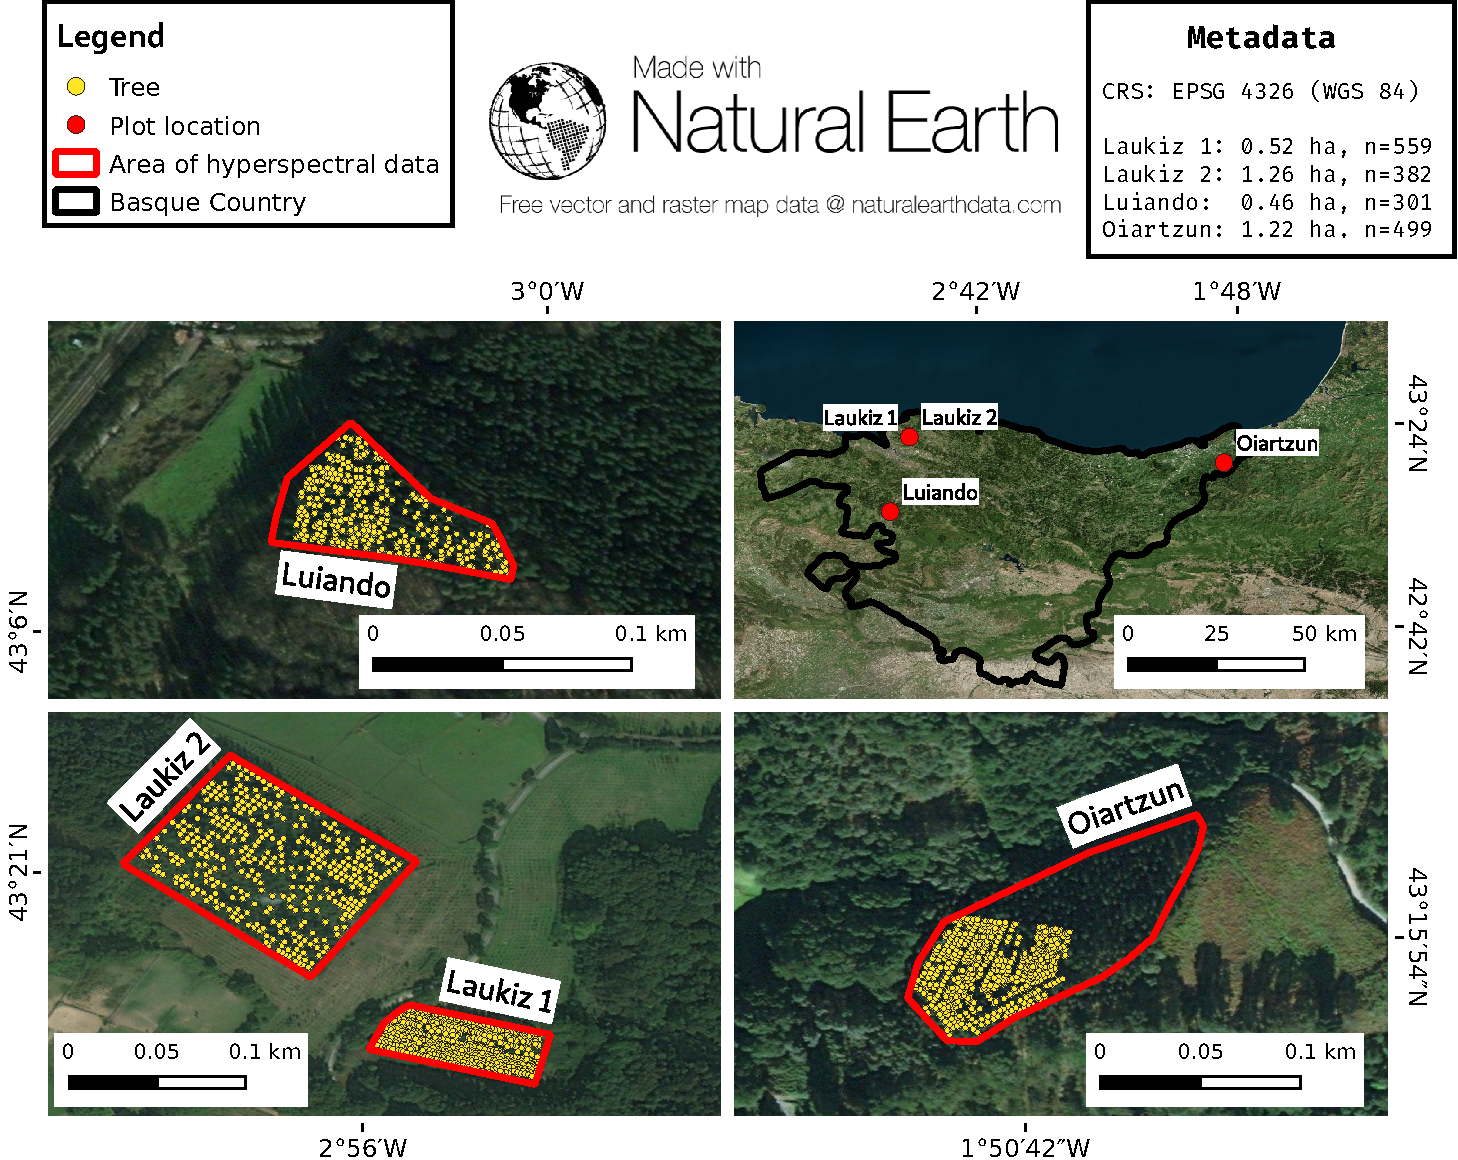
\includegraphics[width=\textwidth] {study_area_hyperspectral.pdf}}
		\caption{Information about the plot locations, the area of hyperspectral coverage and the number of trees per plot.}
		\label{fig:study_area}
	\end{center}
\end{figure}

\subsection{Hyperspectral data}

The airborne hyperspectral data was acquired during two flight campaigns on September 28th and October 5th 2016, both around 12 am.
The images were taken using a AISAEAGLE-II sensor.
All preprocessing steps (geometric, radiometric, atmospheric) have been conducted by the \ac{ICGC}.
The first four bands are corrupted, leaving 122 bands with valid information.
Additional metadata information is available in Table 1:

% parameter limits
\begin{table}[t!]
\centering
\caption[t]{Specifications of hyperspectral data.}
\begingroup\footnotesize
\begin{tabular}{ll}
	\\
	Characteristic         & Value                               \\
	\hline
	Geometric resolution   & 1 m                                 \\
	Radiometric resolution & 12 bit                              \\
	Spectral resolution    & 126 bands (404.08 nm - 996.31 nm)   \\
	Correction:            & Radiometric, geometric, atmospheric
\end{tabular}
\endgroup
\label{tab:hyperparameter_limits}
\end{table}

\section{Methods}

For all analysis steps we used the open-source statistical programming language R \citep{R_core}.
The algorithm implementations of the following packages have been used: \textit{xgboost} \citep{chenXGBoostScalableTree2016} (\textit{xgboost}), \textit{kernlab} \citep{kernlab} (Support Vector Machine) and \textit{glmnet} \citep{glmnet} (Ridge Regression).
We used the R package \textit{mlr} for all modeling related steps.
It provides a standardized interface for a wide variety of statistical and machine-learning models in R simplifying essential modeling tasks such as hyperparameter tuning, model performance evaluation and parallelization \citep{bischlMlrMachineLearning2016}.

\subsection{Derivation of indices}

To use the full information from the hyperspectral data, we not only calculated all possible vegetation indices that are available in the \textit{hsdar} package (90 in total) but also all possible combinations of \ac{NRI}.
We were interested if NRIs of arbitrary band combinations will have a substantial positive effect on the predictive power of the fitted model.
The NRI were calculated using the following formula:

\begin{equation}
	NRI_{i,j} = \frac{b_{i} - b_{j}}{b_{i} + b_{j}}
\end{equation}

\noindent
where $i$ and $j$ are the respective band numbers.

\bigbreak

To account for geometric offsets (which were reported with up to 1 m), we used a buffer of two meters around the centroid of the respective tree.
The mean value of all pixels touched by the buffer was assigned as the final value for each index.
Missing values were removed from the mean value calculation.
In total, 7875 Normalized Ratio Indices NRI were calculated ($\frac{125*126}{2}$).
Due to four corrupted bands and other numerical problems, some indices returned \texttt{NA} for specific observations.
These indices were removed from the dataset, leaving a total of 7471 variables without missing values.

\subsection{Benchmarking of algorithms}

Three algorithms (\textit{xgboost}, \textit{\ac{SVM}}, \textit{\ac{RR}}) were benchmarked on predictive performance.
Besides the well-known \ac{SVM} algorithm \citep{Vapnik1998} we also used \textit{xgboost} which is ensemble method relying on the idea of tree boosting that gained a lot of attention in recent years \citep{chenXGBoostScalableTree2016}.
We also added penalized L2 (Ridge) regression to the portfolio due to its ability to handle highly correlated covariates (REFERENCE).
The probably most popular machine-learning algorithm, Random Forest \citep{Breiman2001}, was not considered for this study: Due to the high number of variables, model fitting times in the range hours for a single model fit were not practicable for this work.
These high fitting times are caused by hyperparameter \texttt{mtry} which scales with the number of variables \citep{Probst2018b}.
After the selection of the best model, we checked if the winning algorithm can achieve a similar performance when using only the most important variables compared to using all variables.
This would simplify the spatial prediction a lot as less indices need to be computed from the data used for prediction.
Also, simpler models are always preferred over complex ones (REFERENCE).

\subsubsection{Performance estimation}

\noindent The algorithms were benchmarked in two ways:
1) Using spatial block \ac{CV} on the plot level with each plot serving as the test set once.
This approach results in four performance estimates, one for each fold.
2) Using five-fold five-times repeated spatial \ac{CV} for each plot based on the k-means clustering approach of \cite{sperrorest}.
As the best algorithm of 1) will be used for the spatial prediction, we first conducted the model selection on this setup and only applied the winning algorithm on 2).

% Add figure visualizing both spCV approaches

\subsubsection{Hyperparameter tuning}

\noindent To tune the hyperparameters of the algorithms, we used \ac{SMBO} via the R package \textit{mlrMBO} \citep{mlrMBO}.
This Bayesian approach first composes \textit{n} randomly chosen hyperparameter settings out of a user defined search space.
After these \textit{n} tries have been evaluated, a new hyperparameter setting which is going to be evaluated next is proposed based on a surrogate model.
This strategy continues until a termination criterion, defined by the user, is reached \citep{Hutter2011, Jones1998}.
In this work we used an initial design of 30 randomly composed hyperparameter settings and a termination criterion of 20 iterations, resulting in a total budget of 50 evaluated hyperparameter settings per fold.
The advantage of this tuning approach is that it substantially reduces the tuning budget which is needed to find a setting close to the global minimum compared to methods that do not use information from previous runs such as \textit{random search} or \textit{grid search} \citep{Bergstra2012}.

\subsection{Variable importance}

\noindent To find indices that contributed most to model performance, we used the internal variable importance measure of the \textit{xgboost} algorithm.
The score is calculated by taking the contribution of each feature for each tree in the fitted model.
The higher the score of a variable, the more important it is for the fitted model when making predictions \citep{chenXGBoostScalableTree2016}.
The variable importance measure is automatically computed during model fit.
In contrast to other approaches such as permutation-based ones, the \textit{xgboost} score is composed out of three parts that contribute to the overall importance \citep{chenXGBoostScalableTree2016}:

\begin{itemize}
	\item Gain: The relative contribution of the feature to the model
	\item Cover metric: How often a feature was selected to be the deciding feature in a tree for a specific observation
	\item Frequency How often a feature occurs in all trees of the model
\end{itemize}

\noindent The \textit{Gain} features is the most important one among the three.
All measures sum up to one \citep{chenXGBoostScalableTree2016}.

% partial dependence plots??

\section{Results}

\subsection{Plot characteristics}

% defoliation boxplots
\begin{figure} [t!]
	\begin{center}
		\makebox[\textwidth]{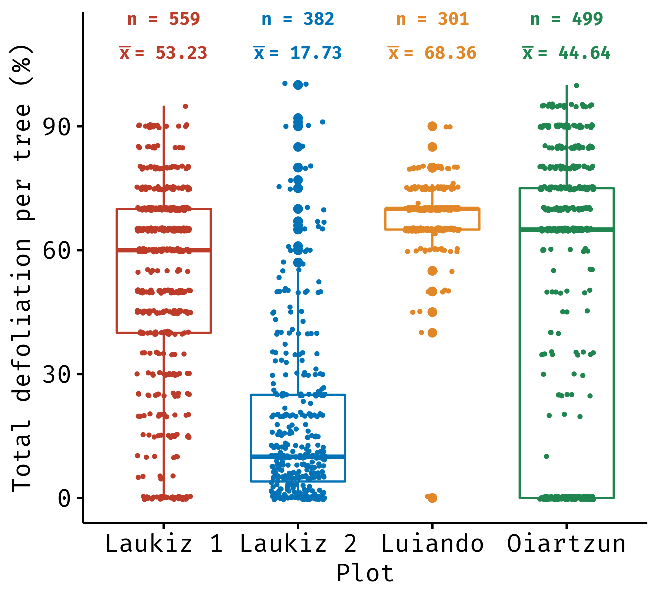
\includegraphics[width=0.7\textwidth] {boxplot_defol.pdf}}
		\caption{Descriptive statistics of the response variable \textit{defoliation}.}
		\label{fig:defol_boxplots}
	\end{center}
\end{figure}

\noindent \textit{Oiartzun} shows the highest defoliation ($\bar{x} = 69.22 \%$) among the plots while \textit{Laukiz 2} is the healthiest ($\bar{x} = 13.54 \%$) (\autoref{fig:defol_boxplots}).
All plots besides \textit{Luiando} show an evenly distributed level of defoliation across the entire plot.

\noindent The high overall degree of defoliation of \textit{Luiando} and \textit{Oiartzun} is also visible in the spectral signatures of the plots (\autoref{fig:spectral_signatures}).
Both plots show lower mean reflectance values around the wavelength range 800 nm - 1000 nm compared to Laukiz 1 and Laukiz 2.
\textit{Oiartzun} is almost completely missing the reflectance drop at around 815 nm that is visible for all other plots but instead shows a higher magnitude for the reflectance increase at around 920 nm.
\textit{Laukiz 2} shows a mean tree density of 61.59 m (\autoref{fig:plot-characteristics}) while all other plots are more dense (34.64 m (Laukiz 1), 33.01 m (Luiando), 34.96 m (Oiartzun)) (\autoref{fig:plot-characteristics}).

\subsection{Predictive performance}

% Performance estimates
\begin{table}[t!]
\centering
\caption[t]{Four-fold block spatial \ac{CV} performances of RR, SVM and xgboost using \ac{RMSE} as the error measure.
	Mean and standard deviation are shown.}
\begingroup\footnotesize
\begin{tabular}{llll}
	RR            & SVM           & xgboost       & xgboost (7 variables) \\
	\hline
	59.10 (22.71) & 36.23 (15.73) & 33.26 (16.61) &                       \\
	\bottomrule
\end{tabular}
\endgroup
\label{tab:model_comparison}
\end{table}

\begin{table}[t!]
\centering
\caption[t]{Predictive performance of \textit{xgboost} using all observations and all variables (All Observations/all variables), all observations and the seven most important variables only (All Observations/7 variables) and observations from specific plots only (Plot level observation/all variables) with \ac{RMSE} as the error measure. The performance estimates for "All Observations" correspond to the fold for which the respective plot was serving as the test set. Column "Plot level observation", shows the mean RMSE estimates at the repetition level of a five-fold five-times repeated spatial CV, scored by using data of the respective plot only.}
\begingroup\footnotesize
\begin{tabular}{llll}
	\\
	Plot/Data & \specialcell{All Observations/ \\{all variables (Block CV)}} & \specialcell{All Observations/         \\ {7 variables (Block CV)}} & \specialcell{Plot level observations/\\{all variables (SpCV)}} \\
	\hline
	Laukiz 1  & 22.03                                                                              & 21.47                          & 19.18 \\
	Laukiz 2  & 51.75                                                                              & 49.94                          & 17.24 \\
	Luiando   & 13.20                                                                              & 15.37                          & 8.30  \\
	Oiartzun  & 32.97                                                                              & 17.62                          & 14.40 \\
	\bottomrule
\end{tabular}
\endgroup
\label{tab:supermodel_performance}
\end{table}

\subsubsection{Algorithm benchmarking}

\noindent The \textit{xgboost} algorithm showed the lowest error (33.26 RMSE) when benchmarking the learners on the complete dataset of all plots (\autoref{tab:model_comparison}).
While the \textit{SVM} performance was only slightly worse (36.23 RMSE), \textit{RR} showed a substantially worse performance than \textit{xgboost} (59.10 RMSE).

\subsubsection{Single models vs. super model}

\noindent When comparing the mean predictive performance of models fitted at the plot level against the performance of the model that was fitted using all data (super model), the plot-level models showed a better performance in all cases (\autoref{tab:supermodel_performance}).
The highest difference between both model types occurred for plot \textit{Laukiz2} with a difference of 34.51 RMSE.

Using only the seven most important variables (\autoref{fig:var-imp}) for the super model showed small increases in performance for \textit{Laukiz 1} and \textit{Laukiz 2}, a small decrease for \textit{Luiando} and almost a reduction of 50\% of the error for \textit{Oiartzun} (32.97 vs. 17.62 RMSE) (\autoref{tab:supermodel_performance}).

\subsubsection{RMSE vs. plot characteristics}

\noindent An increase of the error rate was observed with an increase of descriptive plot measures such as mean point density and the coefficient of variation (based on the response variable \textit{defoliation}) (\autoref{fig:plot-characteristics}).

\begin{figure} [t!]
	\begin{center}
		\makebox[\textwidth]{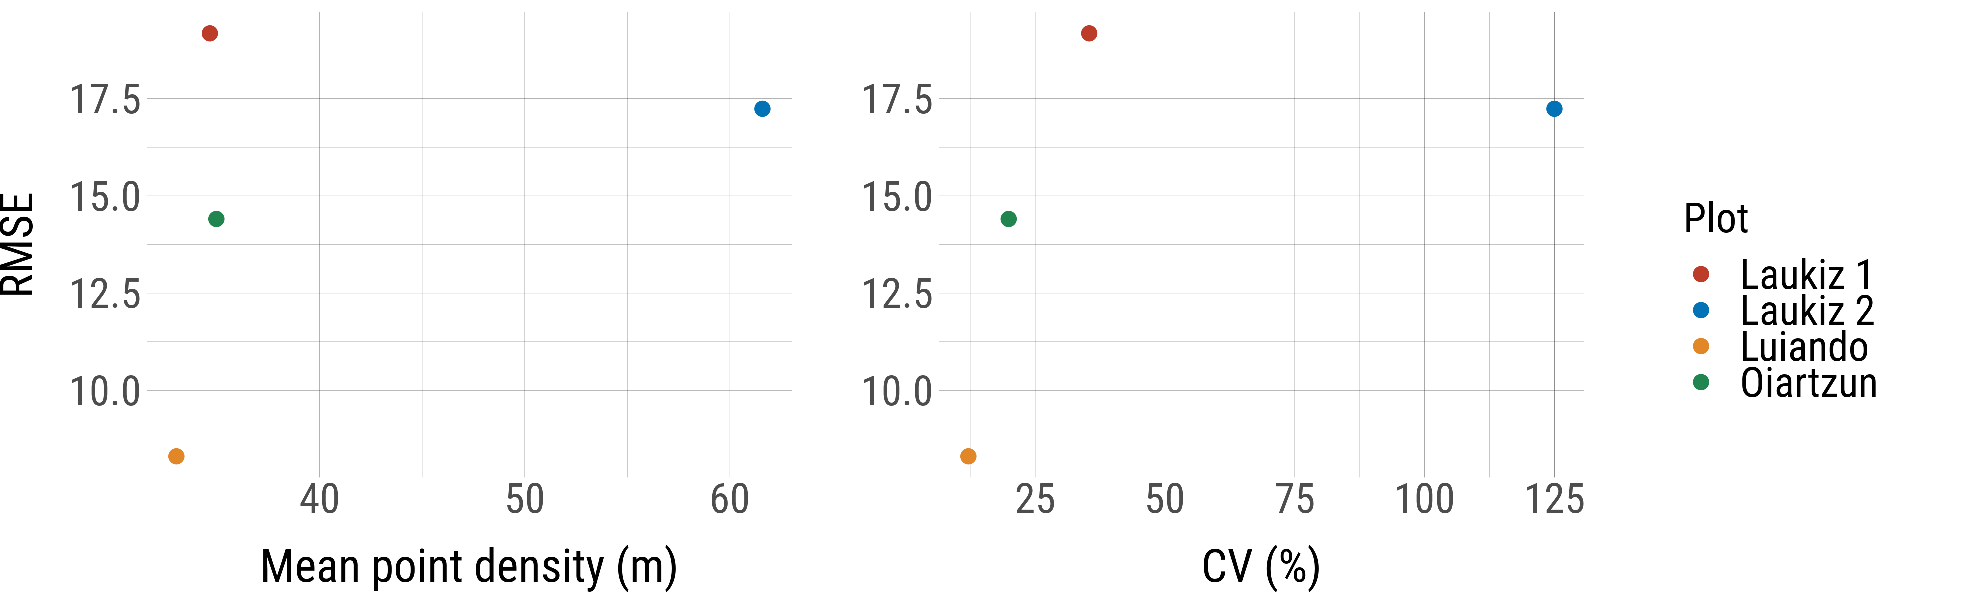
\includegraphics[width=\textwidth] {plot-characteristics.pdf}}
		\caption{RMSE vs. mean point density and coefficient of variation (defoliation).}
		\label{fig:plot-characteristics}
	\end{center}
\end{figure}

\subsection{Variable importance}

\noindent The seven most important features of the super model in this study were vegetation indices with the \textit{EVI} \citep{hueteComparisonVegetationIndices1997} being the most important one (\autoref{fig:var-imp}).

\begin{equation}
	EVI = 2.5*\frac{R_{800}-R_{670}}{R_{800}-(6*R_{670})-(7.5*R_{475})+1)}
\end{equation}

\noindent where $R$ = Reflectance at the respective wavelength.

\bigbreak

\noindent Vegetation index \textit{GDVI} appears three times among the first seven most important features (\autoref{fig:var-imp}) with different \texttt{n} values.
This is because it was computed four times, with \texttt{n} ranging from 1 - 4 \citep{wuEstimatingChlorophyllContent2008}:

\begin{equation}
	GDVI = \frac{R_{800}^n-R_{680}^n}{R_{800}^n+R_{680}^n}
\end{equation}

\bigbreak

\noindent The seven most important features (\textit{EVI}, \textit{GDVI4}, \textit{D1}, \textit{GDVI3}, \textit{GDVI2}, \textit{mNDVI} and \textit{mSR}) show a substantial difference in the importance score compared to all following variables (\autoref{fig:var-imp}).

\begin{figure} [b!]
	\begin{center}
		\makebox[\textwidth]{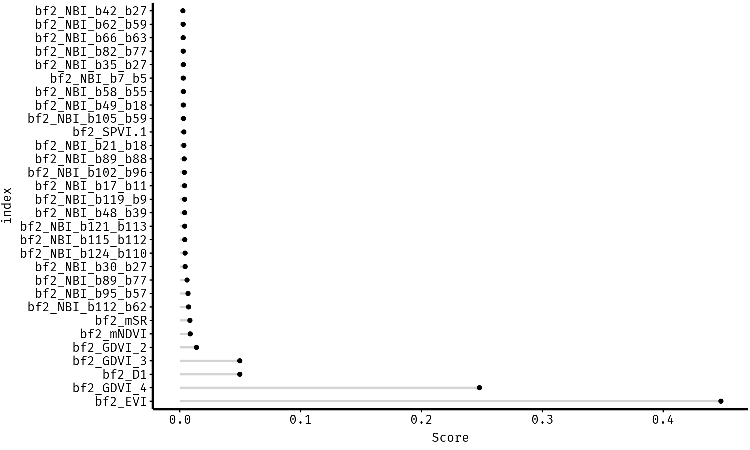
\includegraphics[width = 1\textwidth] {var-imp-xgboost.pdf}}
		\caption{The 30 most important variables as estimated by the internal variable importance measure of the \textit{xgboost} algorithm. The higher the score, the more important the feature.
			"bf2" notes that a buffer of 2 meter was used to extract the variable information to the tree observation. "NRI" means that a normalized ratio index with the subsequent bands was calculated. Features without "NRI" prefix are vegetation indices, e.g. "bf2\_EVI".}. %An overview of the vegetation indices can be found \href{https://rdrr.io/cran/hsdar/man/vegindex.html}{here}.}
		\label{fig:var-imp}
	\end{center}
\end{figure}

\begin{table}[t!]
\centering
\caption[t]{Formulas of the five most important vegetation indices of the super model. $R$ = Reflectance at wavelength, $D$ = First derivation of reflectance value at wavelength.}
\begingroup\footnotesize
\begin{tabular}{llll}
	\\
	Acronym & Name                      & Formula                                                            & Reference                                                 \\
	\hline
	EVI     & Enhanced vegetation index & $2.5*\frac{R_{800}-R_{670}}{R_{800}-(6*R_{670})-(7.5*R_{475})+1)}$ & \cite{hueteComparisonVegetationIndices1997}               \\
	GDVI    & Generalized DVI*          & $\frac{R_{800}^n-R_{680}^n}{R_{800}^n+R_{680}^n}$                  & \cite{wuEstimatingChlorophyllContent2008}                 \\
	D1      & Derivative Index          & $\frac{D_{730}}{D_{706}}$                                          & \cite{zarco-tejadaSteadystateChlorophyllFluorescence2003} \\
	mNDVI   & Normalized DVI*           & $  \frac{R_{800}-R_{680}}{(R_{800}+R_{680}-2*R_{445}}$             & \cite{simsRelationshipsLeafPigment2002}                   \\
	mSR     & Simple Ratio Index        & $\frac{R_{800}-R_{445}}{R_{680}-R_{445}}$                          & \cite{simsRelationshipsLeafPigment2002}                   \\
	\bottomrule
	\multicolumn{2}{l}{\small{* Difference Vegetation Index}}
\end{tabular}
\endgroup
\label{tab:most_imp_vars}
\end{table}

\noindent The best NRI scored rank eight (band 112 and band 62).
All further places up to rank 30 are NRIs.

\subsection{Spatial prediction}




\section{Discussion}

\subsection{Derivation of indices}

\noindent The buffer of 2 m that we used to generate the index value for each observation can be seen critical.
When using no buffer at all, the possibility is high that a pixel value gets assigned to the tree observation that does not spatially match.
Using a buffer of more than 2 meters would increase the probability of merging information from other trees into the pixel value, blurring the actual value of the tree observation.
Thats why in our view using a buffer of 2 m was the best compromise here.

The exact number of contributing pixels to the final index value of an observation cannot be determined as it depends on the location of the tree within the pixel grid.
As the buffer is a circle, it depends on the exact location of a tree observation within a pixel how much surrounding pixels are touched by the circle that will then be used to calculate the final pixel value.
If a tree observation is located at the border of the plot, some directions of the buffer will contain no values and the subsequent index value will be calculated using less pixels than if the tree observation is located in the middle of the plot.

Using a buffer in the first place and the fact that it is unclear how much information from other trees went into the calculation of an index value of a certain observation introduced a bias of an unknown magnitude into the data.
This has to be considered when making interpretations about the outcome of this study.

\subsection{RMSE vs. plot characteristics}

\noindent Relating the modeling error to plot characteristics (mean point density, coefficient of variation) did not show a clear picture: For both comparisons, \textit{Laukiz 2} did not follow the pattern that was observed from the other three plots (\autoref{fig:plot-characteristics}) of having an increase in error with an increase in mean point density and coefficient of variation.

It needs to be considered that we only looked at four plots in this work.
To make a robust statement about a possible relationship between modeling error and plot characteristics, a larger sample size of plots is needed.

\subsection{Predictive Performance}

\subsubsection{Algorithm benchmarking}

\noindent The relatively large difference in performance between \textit{RR} (59.10 RMSE) and the machine-learning models (36.23 and 33.26 RMSE) is remarkable.
\textit{RR} has shown promising performance results in other studies when many highly-correlated predictors were involved (REFERECES).
However, in this study, \textit{RR} was not able to achieve a sufficient performance score compared to \textit{SVM} and \textit{xgboost} even though its hyperparameter $\lambda$ was properly tuned using SMBO.

While \textit{xgboost} shows a slightly better performance than \textit{SVM}, the latter has the advantage of only having two hyperparameters that need to be tuned.
This results in a shorter runtime.
Nevertheless, \textit{xgboost} showed the best performance and was subsequently selected to fit the models on the plot level and for the spatial prediction.

An important point that needs to be considered when interpreting the performance results is that we only related defoliation to indices derived from remote sensing data.
Possible other cofounding factors that could possibly help in predicting defoliation were not considered.
One example here is tree age: The older a tree the more vulnerable it may be to pathogen infections causing defoliation.
However, such predictors would not be available for a spatial prediction scenario and one of the main goals of this study is to relate defoliation to variables that are available on a larger scale (e.g. remote sensing indices).

\subsubsection{Single models vs. super model}

It is expected that models that were trained on the plot level only achieve a better performance than the global model.
The low performance on Laukiz 2 for the super model is most likely due to the difference of this plot to all others: The fitted model on Laukiz 1, Luiando and Oiartzun is not capable of reaching a good performance on the Laukiz 2 prediction data.
This is not surprising as Laukiz 2 shows substantially different plot characteristics compared to all others plots in terms of the distribution of the response variable \textit{defoliation} (\autoref{fig:defol_boxplots}) and the mean point density of trees (\autoref{fig:plot-characteristics}).

The low error for Luiando (8.30 RMSE) for the plot model validates the approach of relating defoliation to vegetation indices and NRI.
The overall error of the super model (33.26 RSME) is expected to decrease if more plots are available for training.
To reach an optimal performance, the fitted model would need to include at least one instance of every plot that shows unique characteristics (i.e. here Laukiz 2 is substantially different to the others).
Possibly more plots showing unique characteristics exists that are not integrated into the fitted model of this work.

An interesting find is that the supermodel with only seven variables shows a better overall performance than the model with all 7471 variables (\autoref{tab:supermodel_performance}).
This leads to the conclusion that adding as many variables as possible to a model will not necessarily improve its performance.
In contrast, too much information can even be problematic for the model as it will have a hard time prioritizing variables.
However, to find the most important variables in the first place and to check for the performance difference, a model with all variables needs to fitted first.
This scenario cannot be generalized and different results may occur for other datasets.
Using a model with only a few predictors does not only simplify prediction tasks but also reduces runtime for hyperparameter tuning and performance estimation.

\subsection{Variable importance}

There are some downsides using the internal variable importance approach of xgboost: Due to the contribution of three different parts to the overall importance score it is complicated to understand why a specific feature was selected.
Furthermore the importance calculation approach is only valid for this algorithm and cannot be compared to others.
Nevertheless, as we only relied on the variable importance for this specific algorithm, using the internal xgboost approach was sufficient for this work.

It is not surprising that vegetation indices are most important for the model as they are most sensitive to changes in vegetation health.
Even though we are not directly looking at vegetation health but using the level of defoliation as a proxy, these indices seem to help the model most deciding whether a tree is defoliated or not.
Vegetation indices can help here in two ways:
1) Trees that show a high level of defoliation do also reflect their bad health status through the remaining foliation.
2) Defoliated trees have more influence of bare ground information in their pixel values and will therefore be classified as defoliated by the model.

Even though no NRI made it among the most important variables in this study (stating that the first seven of this study are the most important ones), it is interesting that all ranks from 8 - 30 are occupied by NRI (\autoref{fig:var-imp}).

Our statement saying that the important indices of this study are the first seven can be seen critical as we only based the selection on a visual inspection of the variable importance results (\autoref{fig:var-imp}).
The decision to make a cut between rank seven and eight was based on a combination of two facts: 1) Using only vegetation indices is easier for large scale predictions using satellites like Sentinel-2 (most NRI cannot be used with it) and 2) the drop in the importance score of the variable importance results (\autoref{fig:var-imp}).
However, based on this statement, we could also have made the cut between rank five and 6 but including the two vegetation indices at rank six and seven will eventually improve the model and does not increase runtime.

\section{Conclusion}

\section{Appendix}

\appendix
% https://tex.stackexchange.com/questions/248704/cross-reference-to-appendix-sections-in-elsarticle-document-class
\gdef\thesection{\Alph{section}} % corrected redefinition of "\thesection"
\makeatletter
\renewcommand\@seccntformat[1]{Appendix \csname the#1\endcsname.\hspace{0.5em}}
\makeatother

\section{Spectral signatures of each plot}

% spectral signatures
\begin{figure} [H]
	\begin{center}
		\makebox[\textwidth]{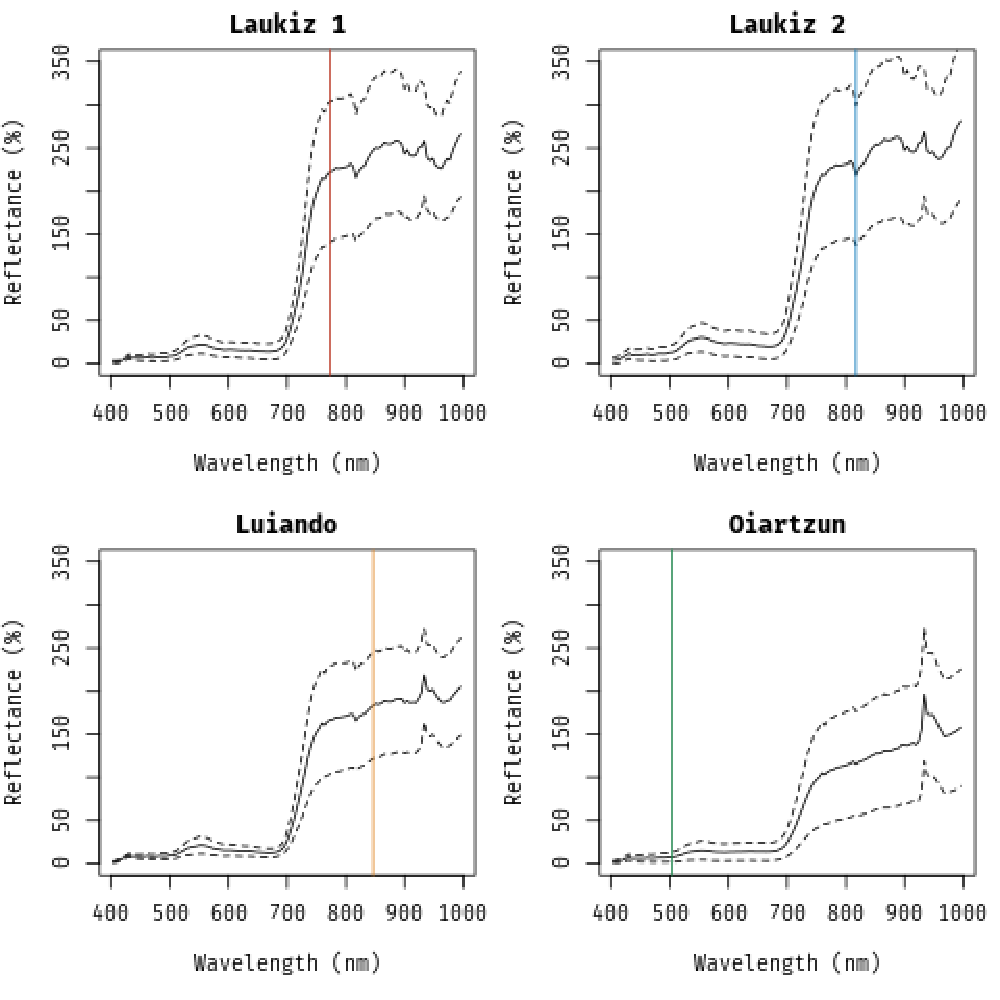
\includegraphics[width=\textwidth] {spectral_signatures.pdf}}
		\caption{Spectral signatures (mean and standard deviation) of each plot.}
		\label{fig:spectral_signatures}
	\end{center}
\end{figure}

\pagebreak

\section*{References}

\bibliography{Biblio_hyperspectral}

\end{document}
